\documentclass{article}
\usepackage[thmmarks, framed]{ntheorem} % ntueorem must come before amsmath, or the cross-reference will not be working
\usepackage[utf8]{inputenc}
\usepackage{graphicx}
\usepackage{booktabs}
\usepackage[a4paper, portrait, margin=1in]{geometry}
\usepackage{amsmath}
\usepackage{amsfonts}
\usepackage{mathtools}
\usepackage{physics}
\usepackage{xcolor}
\usepackage{lmodern} % in conjugate with the fontenc package to prevent pixelisation of output
\usepackage[T1]{fontenc} % to produce the ``dbar'' in thermo
% needed for framed theorems
\usepackage{framed} % or, "mdframed"
%
\usepackage{bm}
\newcommand{\up}{\ket{\uparrow}} % spin up, needs the physics package 
\newcommand{\dn}{\ket{\downarrow}} % spin down, needs the physics package 
\newtheorem{theorem}{Theorem} 
\newframedtheorem{frm-thm}{Theorem} %needed for framed theorems 
\theorembodyfont{\upshape}
\newframedtheorem{frm-res}{Result}
\theorembodyfont{\upshape}
\newframedtheorem{frm-def}{Definition}
\theoremstyle{nonumberplain} 
\theoremheaderfont{\itshape}
\theorembodyfont{\normalfont}
\theoremsymbol{\ensuremath{\square}}
\newtheorem{proof}{Proof}
\title{NST IB Physics B: Thermal Physics}
\date{Lent - Easter, 2023}
\author{Yu Lu}
\begin{document}
\maketitle
\tableofcontents 
\newpage
\section{Mathematical tricks}
A few important results from multivariate calculus include
\begin{itemize}
    \item Chain rule: useful for change of variable $U(x,y)$ into $U(u,v)$
    \[
        \left(\frac{\partial U}{\partial x} \right)_y = 
        \left(\frac{\partial U}{\partial u} \right)_v \left( \frac{\partial u}{\partial x} \right)_y
        + \left(\frac{\partial U}{\partial v} \right)_u \left( \frac{\partial v}{\partial x} \right)_y
    \]
    \item Reciprocal rules: useful for changing the subject variable (``dependent variable'')
    \[
        \begin{aligned}
            \left(\frac{\partial X}{\partial Y} \right)_Z &= \left(\frac{\partial Y}{\partial X} \right)_Z^{-1} \\
            \left(\frac{\partial X}{\partial Y} \right)_Z 
            \left(\frac{\partial Y}{\partial Z} \right)_X &
            \left(\frac{\partial Z}{\partial X} \right)_X = -1.
        \end{aligned}
    \]
\end{itemize}

The second reciprocal rule is often useful when a thermodynamic potential is held constant: we just turn it to the numerator. 

This allows us to easily navigate between differentials of different thermodynamic quantities, yet the question remains: what do we know about the quantities themselves? For example, we might know $p(V,T)$ and correspondingly
\[
    \left( \frac{\partial F}{\partial V} \right)_{T} = -p.
\]
The best we can do, then, is to integrate the differential with respect to $V$ and hold the $T$ constant:
\[
    F (V,T)
    = f(T) + \int \left( \frac{\partial F}{\partial V} \right)_{T} \mathrm{d} V
    = f(T) + \int -p(V,T) \mathrm{d} V, 
\]
leaving an undetermined function that only depends on $T$ and up to a constant. 

A ton of partial differentials can be generated from the algebra above, but often many of them have physical meanings or can be converted. For example, temperature derivatives of entropy can be associated with heat capacities:
\[
    \boxed{
    C_V = T \left(\frac{\partial S}{\partial T} \right)_V = \left(\frac{\partial U}{\partial T} \right)_V
    , \qquad 
    C_p = T \left(\frac{\partial S}{\partial T} \right)_p = \left(\frac{\partial H}{\partial T} \right)_p.}
\]

Thermodynamic variables are grouped into conjugate groups $\{V,p\},$ $\{S,T\},$ and $\{\mu ,N\}.$ The partial derivative of one thermodynamic variable with respect to another thermodynamic variable can be converted to another such partial differential using Maxwell's relations. Often, we want to convert such partial differentials into the conjugate pair $\{V,p\}$ in questions involving gas because the equation of state relates $V$ and $p$ to $T.$ A systematic approach can be used to spot which relation to use: say we start with 
\(
    \left( \frac{\partial S}{\partial p} \right)_{T}, 
\)
then thermodynamic potential we want to consider will have a total differnetial
\[
    \mathrm{d} B = \pm S \mathrm{d} T \pm x \mathrm{d} p, 
\]
where $B$ is a thermodynamic potential and $x$ is a thermodynamic variable. The potential of interest must then be $G$ with $\mathrm{d} G = -S\mathrm{d} T + V \mathrm{d} p,$ giving the Maxwell relation of interest
\[
    \left( \frac{\partial S}{\partial p} \right)_{T} = 
    -\left( \frac{\partial V}{\partial T} \right)_{p}. 
\]

The partial differential of a thermodynamic potential with respect to one thermodynamic variable could be identified as another thermodynamic variable. This is only true if the two are natural variables of the potential. For example, because \(\mathrm{d} G = -S\mathrm{d} T + V \mathrm{d} p,\) we can identify
\[
    \left( \frac{\partial G}{\partial T} \right)_{p} = -S, 
    \qquad
    \left( \frac{\partial G}{\partial p} \right)_{T} = V.
\]
\section{The zeroth and the first law}
\subsection{The zeroth law}
An isolated system will eventually display no noticeable change in the macrostate variables, coming to a state called \textit{equilibrium}. The zeroth law states that temperature is a function of macroscopic state only. Specifically, it states that thermal equilibrium is transitive. Consideration of this on three bodies in equilibrium allows us to define temperature $\theta(p,V)$ as a function of state. One possible form is the ideal gsa temperature 
\[
    T = \frac{p V}{N K_B}, 
\]
but to show that this \textit{is} the thermodynamic temperature $\theta(p,V)$ requires the second law. 

\subsection{The first law}
The first law states that energy is a function of state. It can be stated without introducing anything new that the amount of work required to change an isolated system from state 1 to state 2 is path independent, motivating the internal energy 
\[
    \mathrm{d} U = \mathrm{\dj} q + \dj w,  
\]
where $\mathrm{d} U$ is a state variable, but $\dj q$ and $\dj w$ \textit{individually} are not. For a gas in a quasi-static change, 
\[
    \dj w = - p \mathrm{d} V,
\]
which is not an exact differential, and thus is path dependent. Mathematically, this means that $w$ cannot be properly defined (or as a function of state).

For an ideal gas, the internal energy is a function of $T$ only. For a monatomic gas, $U = 3 N k_B T /2$ (three KE modes). For a diatomic gas, $U = 5 N k_B T /2$ under low temperature (six KE modes, but rotation around the radial vector connecting their COM is prohibited, since we assume them to be point masses) or $U = 7 N k_B T /2$ under high temperature (plus one KE and one PE from vibration). 

The heat capacity of gas is defined as the total derivative
\[
    C_x = \left. \frac{\dj q}{\mathrm{d}T} \right \vert_x = \left. \frac{\mathrm{d}A}{\mathrm{d}T} \right \vert_x, 
\]
where $A$ is a suitable function of state (usually found from the first law). Then, we just need to express $A$ with $x$ being one of its natural variable and compute the partial derivative 
\(
    \left( \frac{\partial A}{\partial T} \right)_{x} 
\)
from chain rule. 

For example, it can be shown that
\[
    C_p = C_V + \left[ \left( \frac{\partial U}{\partial V} \right)_{T} + p\right] \left( \frac{\partial V}{\partial T} \right)_{p} 
\]
and 
\[
    C_{p,m} = C_{V,m} + R
\]
for ideal gas. 
We also define
\[
    \gamma \coloneqq C_p / C_V
\]
and the adiabatic expansion of ideal gas gives 
\[
    \mathrm{d} U = -p \mathrm{d} V \implies 
    p V^\gamma  = \mathrm{const}. 
\]

\section{The second law and entropy}
\subsection{The statements}
Microscopically, everything is reversible due to thermal fluctiation. Macroscopically, things are irreversible if we cannot restore the motion of every microscopic particle (like in a lens). However, assuming that we move the system infinitesimally at a time in the absence of dissipation, macroscopic reversibility is possible (the fluctuation will bring it towards equilibrium). 

At its heart, the second law dictates the arrow of time of irreversible changes: what is done cannot be undone, ergo, the second law breaks the time-reversal symmetry. It is often stated in two different ways: 

\begin{itemize}
    \item \textit{\`{A} la} Kelvin: No process is possible whose \textit{only} effect is the \textit{\textbf{complete conversion of heat to work}}.
    \item  \textit{\`{A} la} Clausius: No process is possible whose \textit{only} effect is to transfer heat \textit{\textbf{from a colder to a hotter body}}. 
\end{itemize}


Reversibility of a process, in the absence of external work, is determined by states of the system only, motivating a state variable characterising reversibility. In other words, reversibility requires
\begin{itemize}
    \item Quasi-static process: the system comes to equilibrium at every stage of the change such that we can describe every stage of the system by the macroscopic variables $(p,V).$ (Essentially, a process that can be fully described by a curve on the $p-V$ diagram)
    \item Absence of dissipation: there is no sources of friction etc. 
\end{itemize}

Suppose we go through a closed path in the $pV$ diagram, then that means at least some parts of the process is irreversible. Assuming everything is quasistatic, then there must be some form of dissipation process. In our context, this is usually due to a temperature gradient between objects. Thermal contact with a reservoir of different temperature essentially breaks the time-reversal symmetry (now the temperature gradient marks the direction of irreversibility). This can be thought as some kind of hysteresis. 

A quasistatic process can be regarded as a process that can be made to go arbitrarily slowly. For example, we have no control over the rate of Joule expansion, making it \textit{\textbf{not}} quasistatic. Similarly, the free motion of a piston in a pressure gradient is also not quasistatic: the piston would accelerate, making it impossible to go arbitrarily slowly. In this case, the pressure wave from the piston disturbs the equilibrium assumption. To make the piston move slowly, we need to include a friction, which can be added as work done on the system or heat dissipated. 

\subsection{Heat engines and the temperature scale}
Carnot engine is a cyclic reversible heat engine, comprising of two isotherms connected by two adiabats. In a cycle, it draws heat $Q_H$ from the hot reservoir and expels heat $Q_C$ from the cold reservoir, with the rest $W = Q_H - Q_C$ being converted to work. By relying on the second law and reversibility of a carnot engine, it can be shown that
\begin{itemize}
    \item There are no super-Carnot engines in terms of heat efficiency 
    \[
        \eta  = \frac{W}{Q_H} = 1 - \frac{Q_C}{Q_H}.
    \]
    In other words, a Carnot engine produces the most work for a given $Q_H.$
    \item All reversible heat engines are Carnot and have the same efficiency $\eta(T_H, T_C).$
\end{itemize}

It is intuitive to see that the only reversible heat engine connecting two reservoirs is a Carnot engine comprising of two adiabatic processes and two isothermal processes because there must be no temperature gradient between the system and the reservoir as far as heat flow is concerned. For example, the Otto cycle comprises of two adiabatic processes and two isochoric processes. Since temperature of the system changes during the isochoric processes, there must be a temperature gradient between the system and the reservoir during heat exchange, bringing about irreversibility. Similarly, when there is a temperature gradient, there must be no heat flow, i.e. the process is adiabatic if it is reversible. 

To calculate the efficiency of a heat engine, we usually use the two adiabats to relate the ratio of volumes and calculate the heat flow from the other two processes (usually isothermal, isobaric, or isochoric).

We could also run a heat engine backwards to make it a heat pump ($\eta = Q_H / W$) or a refrigerator ($\eta  = Q_C / W$). The efficiency of both scales as $(T_H - T_C )^{-1}$ and can thus be greater than 1. For practical purposes, the efficiency of a heat pump is always larger than unity, since otherwise we can just heat the source by dumping all the work as heat without any difficulties (converting orderly energy to unordered energy).

By combining several Carnot engines together, it can be shown that the efficiency of a Carnot engine must take the form
\[
    \eta = 1- \frac{f(\theta_C)}{f(\theta_H)},
\]
which, without loss of generality, allows us to define the thermodynamic temperature in terms the carnot efficiency 
\[
    f(\theta ) = \theta \implies \eta  = 1 - \frac{\theta_C}{\theta_H}.
\]
Consider a Carnot engine driven by ideal gas, then, gives
\[
    \boxed{\frac{Q_1}{T_1} = \frac{Q_2}{T_2}} \implies  
    T = \theta
\]
as promised. 

\subsection{Clausius' theorem and Entropy}
From Carnot's cycle, we can conclude that 
\[
    \frac{Q_1}{T_1} = \frac{Q_2}{T_2},
    \quad \implies 
    \oint_{\mathrm{rev} } \frac{\dj q}{T}= 0
\]
along any reversible path, where $\dj q$ is positive for any heat flowing into the system. Since we can always subdivide a Carnot cycle to any arbitrary shape by connecting more isotherms and adiabats around the corner, it is possible to represent any reversible change as a series of Carnot cycles. Therefore, the results above hold for any reversible path in the phase space. It is worth noting that while any path in the $pV$ diagram can represent a reversible change, it is not a sufficient condition for reversibility (essentially, only the quasistatic condition is met). Therefore, it is perfectly fine for the same path in the $pV$ space to represent a reversible change or an irreversible change\textemdash the difference lies in dissipation. In this sense, the ``path-dependence'' in the $pV$ space is not the same as the difference between a reversible and an irreversible change.

The above statement also means that the integral is path-independent in the phase space for a reversible change, motivating us to define the entropy of \textit{the system}
\[
    \Delta S \coloneqq \int \frac{\dj q_{\mathrm{rev} }}{T}
\]
The Carnot's theorem tells us that the irreversible path always ejects more heat into the surrounding, making the integral more negative, thus
\[
    \boxed{\oint \frac{\dj q}{T} \leq 0, \quad 
    \Delta S = \int \frac{\dj q_{\mathrm{rev} }}{T} \geq  \int \frac{\dj q}{T}}
\]
for a general change, with the equality achieved for a reversible change. Therefore, a reversible adiabatic change is also isentropic. Extending our notional box to encompass the universe (which is assumed to be isolated) gives that \(\Delta S_{\mathrm{universe}} \geq 0\) for any change allowed by the second law. 

The entropy $S$ is, as we've seen mathematically, a function of state: a reversible change and an irreversible change following potentially different paths in the $pV$ space lead to the same (likely non-zero) entropy change of \textit{the system}. The reversibility should not matter at this stage, as entropy is \textit{defined} using the heat flow in a reversible change. The difference between a reversible and an irreversible change only lies in the entropy change of the surrounding, which is a function of state of the surrounding. In a reversible change, the entropy change of the surrounding exactly cancels with the entropy change of the system. However, by no means can we find the volume change of the rest of the universe, so this doesn't feel like a state variable to us, as we only have access to state variables of the system. In that regard, it is clear that a reversible change and an irreversible change put the universe into different states. 

More specifically, as the irreversible heat is transferred to the surrounding, the only change in its state function is the enthalpy change, equal to the heat received. To calculate the entropy change of the surrounding, we need to regard it as our new system and subject it to the new system, but we should end up with the same enthalpy change, giving $\Delta S = \frac{q}{T_{\mathrm{surr} }}. $ As a recipe, the entropy change of the universe in an irreversible process can be calculated as
\[
    \Delta S_{\mathrm{universe} } = \int \frac{\dj q_{\mathrm{rev} }}{T_{\mathrm{sys} }} + \sum_{}^{} - \frac{q_{\mathrm{irre} }}{T_{\mathrm{surr} }}, 
\]
where $q$ is positive for heat flow into the system and $q_{\mathrm{rev} }$ is the heat flow of a devised reversible process with the same start and final state. 

\subsection{Adiabatic changes}
The second law can also be stated as the existence of an adiabatic surface (total differential). The adiabatic curve can be either solved by 
\[
    \mathrm{\dj} q = \mathrm{d} U - p \mathrm{d} V = 0 
\]
when $U(p, V)$ is known or by 
\[
    \mathrm{d} S = 0
\]
when the total derivative of $S(p,V)$ is known in analytic thermodynamics.
\section{Analytical thermodynamics}
In thermodynamics, we distinguish between a system and a surrounding. The surrounding is so large such that its intensive variables ($p,$ $T,$ and $\mu $) are regarded as constants. The boundaries between the system and the surrounding can be different nature 
\begin{itemize}
    \item open system: particle and energy flow $\mathrm{d} N,$ $\mathrm{\dj}q,$ and $\mathrm{\dj}w $ allowed
    \item closed system: only energy flow $\mathrm{\dj}q $ and $\mathrm{\dj}w $ allowed 
    \item isolated system: adiabatic $\mathrm{\dj} q = 0$ and $\mathrm{\dj}w  =0,$ but $\mathrm{d} S = 0$ only for reversible changes (think of Joules expansion as a counterexample).
\end{itemize}
The system is said to be in \textit{\textbf{thermal equilibrium}} once the heat flow is stopped. The system and the surrounding together forms an \textit{isolated} system, so any drop of energy in the system is matched by the same amount of increase in the surrounding. The only exception is the entropy, which stays the same or increases for the whole universe. Every change in the surrounding, therefore, can be expressed with only \textit{system variables.}

Unless specified otherwise, it is assumed that only ``$pV$-work'' is done with fixed particle number, so the master equation is 
\[
    \boxed{dU = T \mathrm{d} S - p \mathrm{d} V.} 
\]
\subsection{Thermodynamic potentials}
The internal energy $U(S,T)$ quantifies energy stored in the system that can be converted to work or heat under certain conditions, but its change is expressed in terms of $S$ and $V$ which are not always convenient. Of course, $U$ can encapsulate other forms of energy, such as CoM kinetic energy and gravitational potential energy, so long as they are state functions. Often, we want to study the heat flow or work done in terms of $p$ and $T$ as well. Moreover, the natural variables of $U$ are $S$ and $T$, so we only know complete information about the system if $U(S,T)$ is given (the other two quantities can be worked out by differentiation). Often, however, systems are not expressed in $S$ and $T$, motivating thermodynamic potentials with different natural variables. 

Through Legendre transform, \textit{\textbf{enthalpy}} , \textit{\textbf{Helmholtz free energy}}, and \textit{\textbf{Gibbs free energy}} can be defined as (the natural variables are included in the arguments)

\[
    \boxed{
    H(p,S) = U + p V, \qquad \mathrm{d} H = T \mathrm{d} S + V \mathrm{d} p ;}
\]
\[
    \boxed{
    F(V,T) = U - TS, \qquad \mathrm{d} F = - S \mathrm{d} T - p \mathrm{d} V;}
\]
\[
    \boxed{
    G(p,T) = H - TS = F + p V = U + pV - TS, \qquad \mathrm{d} G = -S \mathrm{d} T + V \mathrm{d} p.}
\]

The $+pV$ terms in Legendre transform can be interpreted as excluding $pV$-work while the $-TS$ terms can be interpreted as reflecting the maximum work extractable (see section \ref{subsec:availability}). Mathematically, thermodynamic variables can be extracted by differentiating these potentials. Moreover, we could arrive at \textit{\textbf{Maxwell relations}} using commuting partial derivatives, such as 
\[
    \frac{\partial ^{2} U}{\partial S \partial V}  = 
    \left( \frac{\partial T}{\partial V} \right)_{S} = 
    -\left( \frac{\partial p}{\partial S} \right)_{V} 
\] 

Sometimes we are interested in flow processes, in which gas with $(p_1, V_1)$ are put into some devices and gas with $(p_2, V_2)$ are ejected. In this case, the first law can be expressed in terms of the enthalpy
\[
    \boxed{H_1 + Q + W = H_2,}
\]
and enthalpy is conserved if no heat or work is given to the system. 

Since $\dj q = T \mathrm{d} S$ for a reversible process, $\mathrm{d} U$ and $\mathrm{d} H$ quantifies the heat exchange under constant volume and pressure. They are conserved for adiabatic processes ($\mathrm{d} S = 0$) under constant volume or constant pressure. 
The heat capacities are easily measurable, and they are defined as
\[
    \boxed{C_x = \left( \frac{\mathrm{\dj}q}{\mathrm{d}T} \right)_x 
    = T \left( \frac{\partial S}{\partial T} \right)_{x}, 
    } 
\]
where $x$ is the quantity held constant. Under constant pressure volume or pressure, these can be related to $U$ and $H$ as
\[
    C_V = \left( \frac{\partial U}{\partial T} \right)_{V},  \quad 
    C_p = \left( \frac{\partial H}{\partial T} \right)_{p}.
\]
For an isentropic change, $dU = \mathrm{\dj} w,$ and $U$ truly behaves like an energy. However, since $T$ are not natural coordinates of $U$ and $H$, these are more useful experimentally. 

In situations with varying particle numbers (such as phase transition), the chemical potential
\[
    \boxed{\mu = \frac{G}{N}}
\]
is often useful. It is related to the total differential of $G$ as 
\[
    \mathrm{d} G = V\mathrm{d} p - S \mathrm{d} T + \mu \mathrm{d} N
     = \mu \mathrm{d} N + N \mathrm{d} \mu. 
\]
Consider a two-phase (or multiple-phase in general) system. At equilibrium, the chemical potential of two phases must be equal ($\mathrm{d} G = 0$), which can be used to solve for the pressure distribution of the isothermal atmosphere (or contact potential) after including the gravitational potential energy in $U.$ The same idea is useful in studying phase transition. 
\subsection{Free energy and availability}
\label{subsec:availability}
By definition, a surrounding is large enough so that its intensive variables $p_0$ and $T_0$ does not change in equilibrium. Then the second law requires
\(
    T_0 \mathrm{d} S \geq  \mathrm{\dj} q,
\)
which can be combined with the first law to yield
\[
    \mathrm{\dj} W_{\mathrm{non-pV} } = \mathrm{\dj} W + p_0 \mathrm{d} V
    \geq \mathrm{d} A,  
\]
where 
\[
    \boxed{A = U + p_0 V - T_0 S,\qquad \mathrm{d}A = \mathrm{d} U + p_{0} \mathrm{d} V - T_0  \mathrm{d} S ,} 
\]
is the availability of the system. Note that this is quite similar to the definition of $G,$ just that $T_0$ and $p_0$ are properties of the surrounding, not the system itself. This leads to differences in their differentials.

If we want to extract work from the system, then $\mathrm{\dj}w $ is negative and $\mathrm{d} A$ gives the maximum amount of work extractable from the system. Under constant temperature and volume, for example, notionally the maximum work that can be harnessed is the drop in potential energy $\Delta U$(consider a mass dropping from a mountain). If this process has intrinsic entropy change (like in a electrochemical reaction), we could allow heat flow from the surrounding and convert it to work till the point that the entropy change of the universe is zero and the process becomes reversible. The maximum work extractable is then given by the drop in $F.$

Similarly, if the system is mechanically isolated with $\mathrm{\dj} w_{\mathrm{non-pV} } = 0, $ we must have
\[
    \mathrm{d}A \leq  0,
\]
Therefore, an isolated system always tries to minimise $A.$ Irreversibility arises during this process, but again this can be harnessed and make the whole process reversible (In a reversible evaporation process ($T$ constant), for example, $\Delta G = 0$, and the maximum work done (including $pV$ work) is $-\Delta F.$) Under different constraints, $\mathrm{d}A $ is equivalent to other thermodynamic variables that we try to extremise. 
\begin{itemize}
    \item Isolated with fixed volume ($\mathrm{d} U = \mathrm{d} V = 0$) \\
    \[
        \mathrm{d} A = -T_0 \mathrm{d} S \implies \underline{\mathrm{d} S \geq 0;} 
    \]
    \item Fixed volume at constant temperature ($\mathrm{d} V = \mathrm{d} T = 0$) \\
    \[
        \mathrm{d} A = \mathrm{d} F \implies \underline{\mathrm{d} F \leq  0;}
    \]
    \item Constant pressure and temperature ($\mathrm{d} p = \mathrm{d} T = 0$) \\ 
    \[
        \mathrm{d} A = \mathrm{d} G \implies  \underline{\mathrm{d} G \leq  0.}
    \]
\end{itemize} 

Under constant $T,$ $-\Delta F$ gives the maximum work done by the system, including any $pV$ work in a reversible process. If no work is done and $V$ is a constant, then the process is irreversible and 
\[
    \mathrm{d} S_{\mathrm{tot} } = -\frac{\mathrm{d} F}{T}.
\]
Under constant $T$ and $p,$ $-\mathrm{d} G$ gives the maximum non-$pV$ work done by the system in a reversible process. If no non-$pV$ work is done, the process is irreversible and 
\[
    \mathrm{d} S_{\mathrm{tot} } = -\frac{\mathrm{d} G}{T}.
\]
Furthermore, if heat flow is allowed in the flow process, then $G_1 = G_2$ when no work is done on the system under constant temperature. 

Why do we define $\mathrm{d} F = \mathrm{d} U - T_0 \mathrm{d} S - S \mathrm{d} T$ in p.p.178 of Blundell, not the normal $\mathrm{d} F = \mathrm{d} U - T \mathrm{d} S - S \mathrm{d} T$? 

\subsection{Examples}
For an ideal gas,
\[
    S(T,V) = n (C_{V,m } \ln T + R \ln (V/n) + S_0), 
\]
The isothermal and adiabatic compressibilities are related by 
\[
    \frac{\kappa _{T} }{\kappa _{S} } = 
    \frac{\left( \frac{\partial V}{\partial p} \right)_{T} }{\left( \frac{\partial V}{\partial p} \right)_{S} }
    =\frac{C_p}{C_V} = \gamma.
\]
The constant pressure and constant volume heat capacities are related by
\[
    C_p - C_V = T \left( \frac{\partial p}{\partial T} \right)_{V} \left( \frac{\partial V}{\partial T} \right)_{p}.
\]
The pressure distribution of an isothermal atmosphere is 
\[
    p(h) = p_0 \exp \left(-\frac{m_r g h}{RT}\right),
\]
which can be obtained from setting the chemical potential $\mu(h)$ to be uniform.
\subsection{Thermodynamics of other systems}
The ideas and techniques of thermodynamics can be used to study other systems with a large number of particles, such as rubber molecules, liquid molecules, or magnetic dipoles. In these systems, instead of (only) having the $-p \mathrm{d} V$ work, other forms of work 
\[
    \mathrm{d} W = X \mathrm{d} x,
\]
may be of interest, such as $\mathrm{\dj} W = - \mathbf{m} \cdot \mathrm{d} \mathbf{B}$ for magnets, $\mathrm{\dj} W = f \mathrm{d} L$ for an elastic rod, or $\mathrm{\dj} W = \gamma \mathrm{d} A$ for a liquid.  
We can also introduce the equivalence of free energy or enthalpy to calculate ``useful work.''

\subsubsection{Elastic rod}
For an elastic rod, the first law becomes
\[
    \mathrm{d} U = T \mathrm{d} S + f \mathrm{d} L. 
\]
For example, the entropy of the change as length at a constant tmeperature as
\[
    \left( \frac{\partial S}{\partial L} \right)_{T} = A E_T \alpha_f = \left( \frac{\partial f}{\partial L} \right)_{T} \left( \frac{\partial L}{\partial T} \right)_{f}. 
\]
This is positive for metallic bars, as pulling the bar distorts the crystal. Notably, for a rubber band, the expansivity $\alpha_f$ is negative, as pulling actually decreases the entropy by aligning the robber molecules. This also means that a rubber band heats up in an adiabatic expansion. 

\subsubsection{Surface tension}
For a liquid, the intermolecular attraction is isotropic in the bulk but points towards the inside of liquid near the surface. This gives rise to surface tension, making 
\[
    \mathrm{\dj} W = \gamma \mathrm{d} A. 
\]
At equilibrium, the pressure difference supports the surface tension (the principle of virtual work):
\[
    \mathrm{d} W = p \mathrm{d} V = \gamma \mathrm{d} A,
    \] 
giving $p - p_{\mathrm{atm} } = 2\gamma /r$ for a droplet. Expansion of the surface area requires injection of heat and would increase the entropy.

\subsubsection{Paramagnetism}
A magnet consists many magnetic spins, pointing up or down. Magnetic susceptability of a sample decreases as temperature increases due to Curies' law, giving 
\[
    \left( \frac{\partial \chi }{\partial T} \right)_{B} < 0
\]
and consequently
\[
    \left( \frac{\partial S}{\partial B} \right)_{T} < 0, \qquad
    \left( \frac{\partial T}{\partial B} \right)_{S} > 0. 
\]
Therefore, isothermal magnetisation emits heat while adiabatic magnetisation heats the magnet up. Microscopically, this is because an external magnetic field aligns the spins, therefore decreasing the entropy. During adiabatic demagnetisation, entropy of the spins increases due to less alignment. However, since the total change of entropy is $0,$ the entropy of phonon (lattice vibration) must decrease, bringing the temperature down.

The combination of isothermal magnetisation and adiabatic demagnetisation can cool a system down to millikelvins. The system is first magnetised in a heat bath of liquid helium to about $4$ Kelvin, after which it is isolated and the magnetic field is brought down. 

Magnetisation of sample brings down entropy (the spins line up with $B$.) Adiabatic demagnetisation works because decreasing field increases entropy due to spins, but adiabatic => entropy of phonons (lattice vibration) decreases, cooling the sample. 
\section{Phase Transition}
\subsection{Real gases}
Ideality of gas assumes that the gas molecules have no volumes and no intermolecular interactions. In reality, the long-range forces (van de Waals force, for example) drag the molecules together and the finite size of molecules reduces the available space for them to jiggle. We thus want to modify the ideal gas law $p_i V_{mi} = R T,$ where the subscript $m$ denotes molar quantity and $i$ denotes ideality. There are different phenomenological models to express $p_i$ and $V_{mi}$ using the measurable $p$ and $V_m$ (note that we assume them to be equal in the ideal gas law). 

To account for the finite size of molecule sizes, we simply let $V_i = V - b,$ where $b$ is a parameter to be fixed, making the available volume less than the actual volume of the container. The \textit{\textbf{van de Waals}} model of real gas accounts for the intermolecular attraction by $p_i = p + a/V_m^2,$ reducing the actual pressure by the long-range attraction. The $1 / V_m^2$ form of the pressure reduction can be rationalised by approximating the net interaction potential $U$ as proportional to the number of particles $\propto n$ multiplied by the number of nearest neighbouring paris $ \propto n/V$ with the strongest interaction: $U = -a n^2 /V$ The associated effective pressure ($p_i + p_{\mathrm{eff}} = p$) can be determined by $-p_{\mathrm{eff}} \mathrm{d}V = \mathrm{d} U,$ giving the equation of state 
\begin{equation}
    \label{eq:vdw-eq}
    \boxed{
        \left( p + \frac{a}{V_\mathrm{m}^2}\right) (V_\mathrm{m}  - b) = RT.
    }
\end{equation}

The $1/V_m ^{2} $ dependence can be justified in a more \textit{ad hoc} fashion by noting that the interaction would have a $n^2$ dependence, one from the number of particle and the other from the strength of interaction one particular particle feels. The division of $V^2$ then naturally comes from making the $n^2$ dependence intensive. 

Eq.\eqref{eq:vdw-eq} cannot be solved explicitly (easily) for $V$, but it is relatively easy to give an explicit expression for $p$ as 
\[
    p(V,T) = \frac{RT}{V-b} - \frac{a}{V^{2}.}
\]
Often we want to use $p$ as our ``subject variable'' by performing the relevant math trick. For example, 
\[
    \left( \frac{\partial V}{\partial p} \right)_{T} = 
    \left( \frac{\partial p}{\partial V} \right)_{T} ^{-1}.
\]

Various thermodynamic quantities can be obtained from Eq.\eqref{eq:vdw-eq} from chain rules and the Maxwell relations. For example, the entropy is
\[
    \begin{aligned}
        \mathrm{d}S &= \left(\frac{\partial S}{\partial T}  \right)_V \mathrm{d}T + \left(\frac{\partial S}{\partial V}  \right)_T \mathrm{d}V  \\
        &= \frac{C_V}{T}\mathrm{d} T + \left(\frac{\partial p}{\partial T}  \right)_V \mathrm{d}V,
    \end{aligned}
\]
where the second line follows from a Maxwell's relation. The equation of state for a van de Waals gas then gives
\[
    S = C_V \ln T + R \ln (V -b) + \mathrm{const},
\]
which is independent of $a$ since entropy only cares about the allowed space for different configurations. We can also evaluate 
\[
    \Delta U = a \left( \frac{1}{V_1} - \frac{1}{V_2}\right),
\]
which is independent of $b$ since it only cares about intermolecular interactions. 

\subsection{Phase transition of gas to liquid}
Eq.\eqref{eq:vdw-eq} is in general cubic in $V,$ as shown in Fig.\ref{fig:vdw-isotherm}, so the isotherms might adopt an S-shaped curve with two extrema. This isn't allowed in \textit{equilibrium} thermodynamics, as the isothermal compressibility 
\[
    \kappa_T = - \frac{1}{V}\left(\frac{\partial V}{\partial p} \right)_T
\]
should always be positive. This means a positive fluctuation in $p$ expands the gas, making it unstable in a positive feedback loop. At equilibrium, the Gibbs free energy would always be minimised in a constant pressure and temperature experiment, moving along $ABC$ in the $G-p$ plot. The turning point $B$ corresponds is multivalued in the $V-p$ plot and can thus be interpreted as \textit{two phases in equilibrium}: the one on the branch with large volume and large compressibility is gas and the other is liquid. It is worth reiterating that this \textit{\textbf{phase transition}} does not emerge in the ideal gas assumption because intermolecular interaction, which is neglected in gas, cannot be neglected in liquid. 

\begin{figure}[ht]
    \centering
    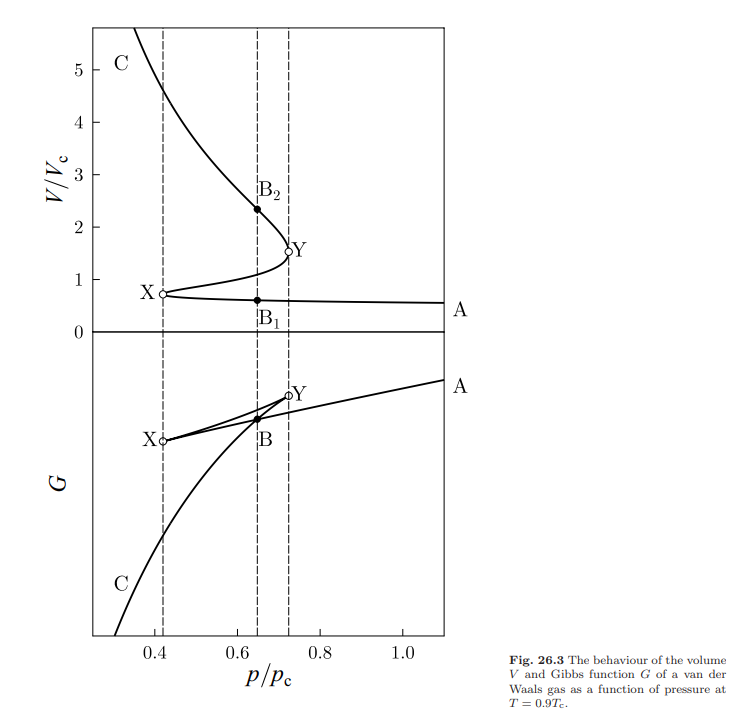
\includegraphics[width=0.8\textwidth]{fig/Blundell-p301.png}
    \caption{Sub-critical van de Waals isotherm. The kinetically feasible path $AXYC$ is different from the thermodynamically stable path $AB_1B_2C$ (Blundell and Blundell, p.p.301)} 
    \label{fig:vdw-isotherm}
\end{figure}

At the transition point $B,$ the Gibbs energy has a double well profile (corresponding to the gas and liquid) with equal depth in the phase space, which becomes biased as one deviates from the equilibrium pressure or volume of coexistence. As one contracts the gas, the gas is stuck at the shallower well that is closer to its original gaseous phase going past the equilibrium volume, giving rise to supercooling along $CY.$ The equilibrium is prevented because of an energy barrier between the two phases and the gas is in a \textit{\textbf{metastable phase}}. However, once a perturbation energy is given, the supercooled gas will return to the equilibrium gas phase, corresponding to a vertical line in the phase diagram. Note that only at $B$ can there be two phases coexisting at equilibrium, and supercooling/superheating are just metastable phases with a higher Gibbs free energy. 

The critical point for phase transition $B$ can be determined by the single-valuedness of $G$ at this point: $G(B_1) = G(B_2). $ Since $G$ is also state function with $V = (\partial G / \partial p )_T$, the change in $G$ along $B_1XYB_2$ must also be 0: 
\[
    \int_{B_1}^{B_2} V  \,\mathrm{d}p =0,
\]
giving the \textit{\textbf{Maxwell construction of equal area}}.  

The coordinates (p, V, T) at the coexistence point $B$ can be used to plot a phase diagram for the gas and liquid. However, the occurrence of a phase transition requires the $S$-shaped profile of isotherms in the first quadrant, which is only feasible up to a critical $T_\mathrm{c},$ mathematically determined by finding the point of inflexion of the isotherm:
\[
    \boxed{
        \left. \left(\frac{\partial p}{\partial V} \right)_T  = 0 \, \right \vert_{T= T_c}, \qquad
        \left. \left(\frac{\partial^{2}  p}{\partial V^{2} } \right)_T  = 0 \, \right \vert_{T= T_c}
    }
\]
There is no phase transition at a higher temperature and the distinction between phases ceases to exist, giving supercritical liquids.

There are other phenomenological models of the real gas. For example, the Dieterici equation takes the boltzmann distribution into consideration, giving 
\[
    p (V_m - b) = RT \mathrm{\exp } \left( -\frac{a}{RT V_\mathrm{m} }\right).
\]

A useful quantity to test ideality is the compressibility factor 
\[
    Z = \frac{pV_\mathrm{m} }{RT}, 
\]
which is unity for the ideal gas. At the critical point, $Z = 3 /8$ for van de Waals gas and $Z \approx 0.27 $ for Dieterici gas. 

Motivated by this factor, we can also model real gas via the virial expansion 
\[
    Z = 1 + \frac{B^\prime }{V_\mathrm{m}  } + 1 + \frac{C^\prime }{V_\mathrm{m}^2  } + \ldots  
    = 1 + \frac{B(T)}{V_\mathrm{m} }, 
\]
where the infinite power series can be terminated at the first term by giving $B(T)$ a temperature dependence. $B = 0$ for an ideal gas, but there is a finite temperature $T_\mathrm{B} $ (called the \textit{\textbf{Boyle temperature}}) at which $B = 0$ again (this is a result of the Leonard-Jones potential). 

\subsection{The law of corresponding states}
The empirical parameters $a$ and $b$ in van de Waals equation differ from gas to gas, but the gas's property can be fully specified by the position and depth of the potential well. Therefore, all gases are the same in the reduced phase coordinates $V/V_c$, $p / p_c$ ,and $T / T_c$ (two degrees of freedom for the intermolecular interaction and one more for the sizes of the particles). However, the quantum mechanical effects prominent in hydrogen and helium breaks this law. 
\subsection{Cooling real gases: Joule-Kelvin expansion}
Ideality of the gas assumes that its internal energy $U$ only depends on the temperature $T$. For an ideal gas, its temperature does not change during a Joule expansion which is adiabatic with no external work, giving 
\[
    \boxed{
    \mu_J \equiv \left(\frac{\partial T}{\partial V} \right)_U 
    = -\frac{1}{C_V} \left( \frac{\partial U}{\partial V} \right)_T}
    = -\frac{1}{C_V} \left[ T \left(\frac{\partial p}{\partial T} \right)_V - p\right]= 0.
\]
For a van de Waals gas, however, it will cool during expansion with 
\[
    \mu_J = -\frac{a}{C_V V^2}, \implies \Delta T = -\frac{a}{C_V} \left( \frac{1}{V_1} - \frac{1}{V_2}\right) <0
\]
Similarly, an \text{isothermal} expansion of van de Waals gas increases its potential energy as 
\[
    \Delta U = a \left(\frac{1}{V_1} - \frac{1}{V_2}\right) >0.
\]

Cooling via Joule expansion is not useful in practice, and we're interested in a constant-enthalpy flow process, thus defining the Joule-Kelvin coefficient 
\[
    \mu_{\mathrm{JK}} = \left(\frac{\partial T}{\partial p}\right)_H. 
\]
From a similar manipulation as that for the Joules coefficient, 
\[
    \mu_{\mathrm{JK}} = -\frac{1}{C_p} \left(\frac{\partial H}{\partial p} \right)_T
    = \frac{1}{C_p} \left[ T\left(\frac{\partial V}{\partial T} \right)_p - V\right]
\]
which can be either positive or negative, though the entropy change is positive definite. Whether we get a cooling or heating from the Joule-Kelvin expansion depends on the exact $p$ and $T,$ but there is a maximum temperature for cooling to happen, known as the \textit{\textbf{inversion temperature}}, below which it is feasible to cool the gas by throttling like this.  

The inversion temperature $T_C$ is the temperature at which $\mu_{\mathrm{JK} } =0,$ determined by 
\[
    T \left( \frac{\partial V}{\partial T} \right)_{p} - V= 0
    \implies 
    -\frac{\left( \frac{\partial p}{\partial T} \right)_{V} }{\left( \frac{\partial p}{\partial V} \right)_{T} } = \frac{V}{T}.
\] 
This is a curve for a real gas with a maximum inversion temperature above which the Joule-Kelvin flow process only heats the gas. But for a van de Waals gas, the inversion temperature is $T_C = 2 T_B$, a constant at all pressure, where $T_B$ is the Boyle temperature ($T_B = \frac{a}{b R}$ for a van de Waals gas).

In practice, we can liquefy different gas in a sequence, starting with the species with highest inversion temperature. In the flow process, high-pressure gas is injected while liquid and gas at atmospheric pressure is ejected. The maximum efficiency of liquefaction occurs when 
\[
    \left(\frac{\partial H_{\mathrm{in}}}{\partial p_\mathrm{in}}  \right)_{T_\mathrm{in}} = 0,
\] along the inversion temperature line with $\mu_{\mathrm{JK} } = 0,$ echoing the line that maximum efficiency is gained only in a reversible process. 

\subsection{Phase Transition}
The continuous change of entropy as temperature increases is characterised by the heat capacity, but often the entropy changes discontinuously at a phase boundary, giving rise to latent heat 
\[
    \boxed{
    L = T_C \Delta S,}
\]
where $T_C$ is the temperature of phase transition. The change in entropy from liquid to vapour can be estimated by the change in density of states 
\[
    \frac{\Omega_{\mathrm{vapour} }}{\Omega_{\mathrm{liquid} }} = \frac{\rho_{\mathrm{liquid} }}{\rho_{\mathrm{liquid} }}^{N_A}, 
\]
giving a rough estimate 
\[
    L \approx 10 R T_C. 
\]

In equilibrium under constant $p$ and $T$, a phase minimises its Gibbs free energy, as discussed in \ref{subsec:availability}. Therefore, if two phases are in equilibrium, $\mathrm{d} G = 0$ for an infinitesimal change from phase 1 to phase 2, giving $\mu_1 = \mu_2.$ This holds for any $p$ and $T$, giving the \textit{\textbf{Clausius-Clapeyron equation}} 
\[
    \mathrm{d} \mu_1 = \mathrm{d} \mu_2, \quad 
    \implies  
    \boxed{
        \frac{\mathrm{d}p}{\mathrm{d}T} = \frac{\Delta s}{\Delta v} = \frac{l}{T \Delta v},  
    }
\]
where the lowercase letters represent quantities per particle. 
\subsubsection{Integration of Clausius-Clapeyron equation}
The Clausius-Clapeyron equation can be integrated under different assumptions to give phase boundaries of different transitions. 

For solid to gas or liquid to gas transitions, we often assume 
\begin{itemize}
    \item $V_{\mathrm{gas} } \gg  V_{\mathrm{liquid} } \approx V_{\mathrm{solid} } \implies \Delta V \approx V_{\mathrm{gas} }$
    \item $p \ll p_{\mathrm{critical}}$ so that the pressure of gas can be modelled by the ideal gas equation $p v = R T;$
    \item (weaker) $L$ is constant along the boundary.
\end{itemize}
These gives
\[
    \frac{\mathrm{d}p}{\mathrm{d}T} = \frac{L p}{R T^{2}}
    \implies  
    \underline{p(T) = p_0 \exp \left( -\frac{L}{RT}\right).} 
\]

For solid to liquid transitions, the ideal gas law is no longer applicable. Instead, we just assume that
\begin{itemize}
    \item $\Delta V$ is constant along the boundary, which can be calculated by the difference in densities;
    \item (weaker) $L$ is constant along the boundary.
\end{itemize}

The assumption of constant $L$ can be relaxed in the liquid-gas and solid-gas transition, as its temperature dependence can be calculated explicitly by noting 
\[
    \frac{\mathrm{d}\Delta S(p,T)}{\mathrm{d}T} = \frac{\mathrm{d}}{\mathrm{d}T} \left(\frac{L}{T} \right) = \frac{1}{T}\frac{\mathrm{d}L}{\mathrm{d}T} - \frac{L}{T^2},
\]
\[
    \implies  
    \underline{L = L_0 + (C_{pg} - C_{pL}) T}. 
\]

\subsubsection{Phase Diagram}
See Blundell and Blundell p.p.327 for an ideal phase diagram. Near the triple point, we should expect 
\[
    L_{sg} = L_{sl} + L_{lg}. 
\]
The volume change from solid to liquid is usually small, giving the steep boundary between solid and liquid. This slope is usually positive, since liquid is less dense than solid, with the notable exception of water due to hydrogen bonding. The phase boundary between solid and gas and liquid and gas takes the same functional form, with a change in the derivative at the triple point due to the change in $L.$ The pressure of the liquid-gas boundary can be interpreted as the ``vapour pressure,'' as 

The phase change from solid to liquid is inherently discontinuous and involve breakage of symmetry. This does not need to be the case for a liquid to gas transition or other transitions. 

\section{Introduction to statistical mechanics}
\subsection{The postulate of equal a priori probability}
A \textit{\textbf{microstate}}  specifies the state (i.e. energy and position) of all particles (e.g. particle 1 is at $x_1$ with energy $E_1,$ and particle 2 is at $x_2$ with energy $E_2\ldots  $) while a \textit{\textbf{macrostate}} specifies collective properties of the system, such as the total energy $E.$ The number of possible microstates corresponding to a macrostate with total energy $E$ can be denoted by $\Omega(E).$ An \textit{\textbf{ensemble}} of several systems contains all the possible microstates, subjected to some constraints:
\begin{itemize}
    \item The microcanonical ensemble: each system has the same fixed energy 
    \item The canonical ensemble: each system is thermally connected to the same large reservoir and the total energy of the systems and the reservoir is fixed. 
    \item The grand canonical: each system can exchange heat and particles with the reservoir. 
\end{itemize}

From the time-reversal symmetry in quantum mechanics, a single isolated system has a conserved energy $E$. Due to interaction, different particles can exchange energy with each other, resulting in the system going through different microstates. The reversal symmetry in such energy exchange means that the probability for each microstate in $\Omega(E)$ is the same, which is known as the \textit{\textbf{postulate of equal a priori probability.}} Furthermore, a microstate in $\Omega(E_1)$ occurs with the same probability as a microstate in $\Omega(E_2).$ This way, we can compute probability distribution of macrostates just based on $\Omega.$

This sheds new light on reversibility of thermodynamic processes. Passive(kinetic) change of a system such as the size of the hole in Joule expansion doesn't change reversibility in equilibrium because they affect the forward and backwards processes simultaneously. Macroscopic irreversibility only occurs because a change in the constraint, such as the position of the poston, that changes the space of possible microstates (the states before change is only a small subset of the states after change). 
\subsection{The Boltzmann factor}
Consider two systems in thermal equilibrium with fixed total energy $E = E_1 + E_2.$ Maximising the total configuration number then gives 
\[
    \frac{\mathrm{d}}{\mathrm{d}E_1} (\Omega(E_1) \Omega(E_2)) = 0, 
    \implies  
    \frac{\mathrm{d}\ln \Omega_1 (E_1)}{\mathrm{d} E_1} =\frac{\mathrm{d}\ln \Omega_2 (E_2)}{\mathrm{d} E_2},
\]
suggesting identifying a statistical temperature scale
\[
    \boxed{\beta = \frac{\mathrm{d}\ln \Omega}{\mathrm{d} E}. }
\]
Note that the temperature $\beta$ already takes the specific form of configuration $\Omega$ into account. 

In the canonical ensemble with total energy $E$, the probability of getting a \textit{microstate} of the system with energy $\epsilon $ a \textit{macrostate} of the reservoir with energy $E - \epsilon$ is $P(\epsilon ) \propto \Omega(E-\epsilon )\times 1.$ Assuming that the temperature $\beta$ of the reservoir (and thus the system, since they are in equilibrium) doesn't change, Taylor expanding $\ln{\Omega}$ gives the Boltzmann factor 
\[
    \boxed{ P(\epsilon ) \propto e^{-\beta \epsilon}}
\]
subjected to normalisation. Note that this does not take the multiplicity of microstates in the system $\Omega_s(\epsilon)$ into consideration since that is not contained in the thermodynamic temperature $\beta.$ The Boltzmann is purely a result of the dropping $\Omega_R(E- \epsilon)$ as the energy of the reservoir drops. 

For a system in equilibrium with reservoir of constant temperature $T,$ the probability distribution of its energy $E$ follows the Boltzmann distribution
\begin{equation*}
    \boxed{
    P(\mathrm{macrostate} \, q) = \frac{1}{Z} g_q e^{-E_q / k T}, \quad 
    Z = \sum_{i=1} g_i e^{-E_i / kT}, }
\end{equation*}
where $Z$ is the partition function for normalisation and $g_q$ counts the number of microstates in the macrostate $q.$ Consequently, its average total energy can be written as
\[
    U = \sum_{i=1}^{} P_i E_i = -\frac{1}{Z}\frac{\mathrm{d}Z}{\mathrm{d}\beta }
    = k_B T^2 \frac{\mathrm{d}\ln Z}{\mathrm{d}T} . 
\]
Note that the zero of energy is arbitrary and shall not affect the form of the spectrum. 

For a low-temperature system, mostly all configurations reside in the ground states and the heat capacity tends to zero (i.e. quantisation of states is significant). Under this case, if we manage to excite a large number of particles into the excited states (population inversion), statistics would eventually force them all back down to the ground state. This forms the working principle of LASER. 

For a high-temperature state, all the states are nearly equally occupied and the heat capacity would tend to a constant. This ``recovers'' the postulate of equal a priori probability, since in the high temperature (by its definition), the reservoir would not feel the increase in the system's energy and all microstates of the system would have an equal a priori probability of occupation. Therefore, a system whose energy spacing is equal or smaller than $k_B T$ can be said to be classical. 

\subsection{Equipartition theorem}
If an \textit{\textbf{independent}} generalised coordinate $u$
\begin{itemize}
    \item is \textit{\textbf{classical}} : with $k_B T$ larger than the spacing between states, so that the sum in $U = \sum_{}^{} P_i E_i$ can be replaced by an integral
    \item has \textit{\textbf{uniform}}  a priori probability: its microstates have a uniform degeneracy $g$,
    \item is associated with a \textit{\textbf{quadratic}}  energy $E = \alpha u^{2}$. This puts a upper limit on $T$ so that no anharmonicity arises. 
\end{itemize}
then the average energy associated with this generalised coordinate is $k_B T /2.$ THis can be applied to many ``modes,'' including positions (Hook potential) and velocities (kinetic energy). 

Two such modes can add, supposing the total energy can be superposed, giving the average total energy of a particle
\[
    \boxed{\bar{E} = \frac{1}{2} N K_B T,}
\]
where the degree of freedom $N$ is the number of such independent quadratic coordinates (a bit different from the conventional degrees of freedom). 

This result is purely classical but applies regardless of other underlying potential in the system. That is, particle would have the same translational kinetic energy everywhere on a potential landscape. This unintuitive result arises because only particles with high KE can make their ways up the potential barrier in the first place, and would on average retain the same KE when they settle down. This can be used to give an upper limit of the rate of a chemical reaction, subjected to hindrance due to viscosity (Brownian motion) and going past the desired product. 

This can also be used to explain the heat capacity of a diatomic gas, with 3 translational modes, 2 rotational modes (no rotation along the axis), and 2 vibrational modes, which are excited in this order due to their decreasing delocalisation (thus smaller curvature of the wavefunction). Note that some species may be able to sustain the temperature to excite all of the modes before dissociation. 

\subsection{The Gibbs entropy}
Armed with the Boltzmann factor, we can give a statistical motivation for the classical entropy defined with reversible heat flow. The change in the total energy of the system with macrostate probability $p_i$ can be written as
\[
    \mathrm{d} \expval{U} = \sum_{i=1}^{} \mathrm{d} (p_i E_i) = \sum_{i=1}^{} E_i \mathrm{d} p_i + p_i \mathrm{d} E_i . 
\]
In a \textit{\textbf{reversible}} process, we can associate the first term as the heat flow $\dj Q$ to change the occupation of the same energy states $\ket{\phi}$ and the second term as the work done $\dj w $ to alter the states themselves $\ket{\phi} \to \ket{\phi^\prime }$. If the process is adiabatic ($\dj Q = 0$) (for example, by contracting a box very slowly), then the energy eigenstates changes continuously but occupation of these states remains constant. The adiabatic expansion of monatomic gas $T V^{-2 /3} = \mathrm{const} $ can be recovered. 

In this context, an adiabatic process avoids excitation of irreversibility by decomposing a wavefunction into new states. This requires to motion to be sufficiently slow than than the local equilibrium timescale of molecules (around $10^{-10} s$). Note that adiabatic processes in quantum mechanics may not be classically adiabatic ($\dj Q = 0$): it is merely a synonym for reversibility. It provides a powerful way of manipulating quantum states. 

The classical definition of entropy can be written as
\[
    \mathrm{d} S = \frac{\dj Q_{\mathrm{rev} }}{T} = - \frac{\sum_{i=1}^{} k_B T \ln(p_i / Z) \mathrm{d} p_i}{T},  
\]
giving 
\[
    \boxed{S_{\mathrm{Gibbs} } = -k \sum_{}^{} p_i \ln{p_i} = -k \ln p_{\mathrm{TAGM} } ,}
\]
where 
\[
    p_{\mathrm{ATGM} }  = \lim_{N\to \infty } \sqrt[N]{\Pi p_i} = p_i^{p_i}
\]
is the geometric mean of $p_i$ if we observe the system for a long time. The inverse of this average probability gives the effective number of microstate of a system. 

The geometric mean is always larger or equal than the average mean $\frac{1}{N},$ which would give the familiar boltzmann entropy
\[
    \boxed{S_{Boltzmann} = k_B \ln \Omega.}
\]
The second law and the postulate of equal a priori probability tell us that the system always evolve to equally occupy all possible microstates until any microstate \textit{available} has the same time-averaged probability. Consequently, the entropy always rises in this equilibrating process and eventually converges to the Boltzmann entropy in equilibrium for a isolated system (if it's connected to a reservoir, the probability will follow the Boltzmann distribution). We can explain irreversible processes as the motion of constraints open up new available microstates.

If the system is connected to a reservoir and the allowed states are not degenerative, we could instead approximate the Gibbs entropy by an integral
\[
    S = - k \int g(E) p(E) \ln{p(E)} \mathrm{d} E,
\]
where $p(E)$ is the rapidly decaying Boltzmann factor and the degeneracy of the system $g(E)$ is a rapidly rising factor for a large system. As a result, $g(E) p(E)$ is strongly peaked at an average energy. Therefore, in the limit of a large system, we can only observe microstates over a short range of energy $\Delta E$ and the Gibbs energy can be well approximated by the Boltzmann entropy, with an error on the order of $k\ln{\Delta E}.$

\subsection{The third law}
Experimentally, it has been shown that all systems \textit{in internal equilibrium} has the same entropy at absolute zero ($\Delta H \to \Delta G$ asymptotically as $T \to 0$). Quantum mechanically, this is because the interaction between particles cannot be neglected as $T\to 0,$ thus splitting up degenerate states. Therefore, at $T=0,$ there should be a unique system ground state. Sometimes two phases can have exactly the same energy, then the third law tells us that the latent heat for transition must go to zero. 

This means the heat capacity and thermal expansion goes to zero near the absolute zero, and graphically (TS diagram) it can be shown that we cannot cool a system to absolute zero in a finite numbers of steps because all states have the same entropy at absolute zero. 

\section{Thermodynamics of radiation}
\subsection{Radiation in thermal equilibrium}
\label{subsec:blackbody-radiation}
Consider a cavity at temperature $T$ in thermal equilibrium. The atoms on its wall jiggles around due to thermal motion and hence produces electromagnetic radiation which exists as standing waves with finely-discretised wavevectors in the cavity characterised by a spectral energy density $u_\lambda (\lambda , T).$ Since the cavity cannot do work on the photons, time reversal symmetry dictates that the energy transferred between any two cavities at the same temperature $T$ in any spectral interval must be equal in either directions (otherwise there will be a net flow of heat in equilibrium), known as detailed balancing. In other words, the spectral energy density $u_\lambda(\lambda, T)$ only depends on these two parameters and is a universal function. 

There will be a photon flux exerting radiation pressure on the wall. For a cavity with photon volume density $n$ and energy volume density $u,$ photons can hit the wall with angle to the normal $\theta \in [0, \pi / 2]$, coming from a cylinder of height $c \mathrm{d} t \cos{\theta}.$ Thus, the total number of photons hitting an area $\Delta A$ in time $\Delta  t$ is 
\[
    \Delta N = \Delta A \Delta t \int_{0}^{\pi /2 } (c \cos \theta) n \frac{\mathrm{d} \Omega / \mathrm{d} \theta }{4\pi }\,\mathrm{d}\theta   \implies \boxed{\mathrm{Flux} = \frac{1}{4} n c }. 
\]
Consequently, the radiation flux per unit area (intensity) is 
\[
    I = \frac{1}{4} u c, \quad I_{\lambda} = \frac{1}{4} u_\lambda c.
\]

To maintain thermal equilibrium, any radiation absorbed by the wall must eventually be emitted, perhaps as another photon at some later time. In other words, \textbf{the absorbed energy equals the emitted energy} (what comes in must go out) and the wall cannot stop the flow of radiation. Suppose the spectral density of emitted radiation is $e_\lambda$ and that of absorption is $\alpha_\lambda,$ this gives the \textit{\textbf{Kirchhoff's law}} 
\[
    \boxed{
        \frac{e_\lambda }{\alpha_\lambda} = e^{\mathrm{blackbody} }_{\lambda} = \frac{1}{4}u_\lambda(\lambda, T) c, 
    }
\]
where the right hand side is a universal function of $\lambda$ and $T.$ Good absorbers are also good emitters, and a blackbody is perfect at both. 

The radiation pressure of any cavity is therefore the same as that for a perfect reflector, since all photons are eventually reflected off its surface, giving a momentum exchange of $2 \varepsilon \cos{\theta} / c$ per photon. Therefore, the radiation pressure is simply the flux of particles multiplied by the momentum exchange integrated over all possible energy and angles
\[
    p = \int_{0}^{\infty} \int_{0}^{\pi/2}  \frac{2 \varepsilon \cos{\theta}}{c}  \left( c \cos \theta n \frac{\mathrm{d} \Omega / \mathrm{d} \theta }{4\pi } \right) \,\mathrm{d}\theta   \,\mathrm{d}\varepsilon \implies \boxed{p = \frac{1}{3}u,}   
\]
where it is clear that the spectral density doesn't matter. 

Note that all the calculation in this section assumes the source is point-like with a uniform angular distribution of velocities. The geometric factor would be different for a beam of light, which is quite straightforward with
\[
    I = u c = \sigma T^4, \quad p = u. 
\]

\subsection{Classical thermodynamics of photon gas}
The collective behaviour of photons in a cavity can be studied like a gas, using the machinery of classical thermodynamics. Specifically, under constant temperature (such that the number of photons doesn't change)
\[
    U(T(N),V) = u(T) V \implies \left( \frac{\partial U}{\partial V} \right)_{T} = u. 
\]
Thus the master equation with $\mathrm{d} N = 0$ and the Maxwell relation gives
\[
    u = \frac{1}{3}\left(T \frac{\mathrm{d}u}{\mathrm{d}T} - u \right) \implies u = A T^4,
\]
and the emission intensity thus follows the \textit{\textbf{Stefan-Boltzmann law}} 
\[
    \boxed{I = \frac{1}{4} A c T^4 = \sigma T^4,}
\]
and the total power is simply the intensity multiplied by the surface area. Far away from a point source, we can treat the wavefront as spherical with the distance being travelling as its radius of curvature. 

We can formulate an ``equation of state'' for such gas as 
\(
    p = A T^4 /3 .
\)
With the entropy per unit volume being
\[
    s = \int_{0}^{T} \frac{\dj q}{T} = \int_{0}^{T} \frac{\mathrm{d}u}{\mathrm{d}T}  \,\mathrm{d}T = \frac{4}{3}A T^3,   
\]
it can be established that the chemical potential
\[
    \mu \propto \frac{G}{V} = u + p - T s = 0. 
\]
In other words, merely changing the number of photons doesn't increase entropy of the system because we don't need to ``borrow'' them from a reservoir: we just create them. The zero chemical potential reflects the nature of photons as a quasiparticle that is essentially a packet of energy, so a non-zero chemical potential would double count its energy. Similarly, the chemical potential of a phonon is also zero. 

Increasing the size of the box increases the total radiation energy inside. During expansion, the wall emits photons at the same rate but the number of photons bouncing off the retreating wall decreases (but $v < c$ so there are always photons bouncing off the wall). As a result, the extra photons emitted from the wall populate the expanded cavity with the same density, and thus expanding a cavity increases the number of photons inside. 

\subsection{The black-body distribution}
Classical thermodynamics can determine $u(\omega)$ up to a constant of proportionality, which can only be determined from statistical mechanics. The derivation greatly parallels that for phonons in the Debye model: the standing wave modes of the cavity are allowed, giving a orthorhombic lattice of allowed states. This can be multiplied with the dispersion relation $\omega  = c\left\vert \mathbf{k} \right\vert $ to give the density of states in $\omega$
\[
    \boxed{g_\omega(\omega ) \propto \omega ^{2},} \quad \Leftrightarrow \quad g_\lambda(\lambda) = \lambda^{-4}. 
\]
Each standing wave mode at frequency $\omega$ has an average energy $\expval{u(\omega)}$ according to Bose-Einstein distribution
\[
    \boxed{\expval{u(\omega)} = \frac{\hbar \omega}{\exp(\hbar \omega / k T) - 1}},
\]
so the overall energy density just follows the Planck distribution
\[
    u(\omega, T) \propto \frac{\omega ^3}{\exp(\hbar \omega  / kT) - 1}.
\]
The only difference between this and ths Debye model is that there is no upper bound on the frequency and there are only 2 polarisation states, not 3, for each mode in the $k$ space. It can be seen that temperature doesn't change the overall functional form, and the maximum spectral density occurs at $\lambda T = \mathrm{const} $ for different temperatures. 

The form of $u_\omega$ can relate the Einstein A and B coefficients. For a two level system with the energy difference equivalent to a photon of frequency $\omega$ and connected to a radiation bath with spectral energy density $u_\omega,$ three processes can occur: 
\begin{itemize}
    \item Spontaneous emission of a photon with probability $N_2 A_{21};$
    \item Absorption of a photon for the transition from 1 to 2 with probability $N_1 B_{12} u_\omega;$
    \item The reverse of the above: absorption of a photon, but the system transits from 2 to 1 to emit a photon of the same energy, and re-emit the absorbed photon, with probability $N_2 B_{21} u_{\omega}$ (stimulated emission).
\end{itemize}
In the steady state, there is no net transfer between the two states, 
\[
    N_2 B_{21} u_{\omega } + N_2 A_{21} = N_1 B_{12} u_\omega, 
\]
which can be used to show that population inversion 
\[
    \frac{N_2}{g_2} > \frac{N_1}{g_1}
\]
is required to achieve a net gain in laser, where $g$ is the degeneracy. 

\section{Kinetic gas theory}
\subsection{Maxwell Distribution}
The kinetic gas theory assumes that particles only exchange energy via collisions, so it is valid to trace the trajectory of one particle and regard all the others as reservoirs, thus applying the boltzmann distribution to give the relative probability of one \textit{velocity microstate} 
\[
    f(v) \propto \exp(- m v^{2} / 2 k T), 
\]
centring at the origin. Assuming the allowed states are uniform in the momentum space, the degeneracy of microstates is then the area of a spherical shell in the momentum space, giving the (non-normalised) Maxwell distribution of \textit{speed}
\[
    \boxed{P(v) \propto v^2 \exp\left(- \frac{mv^{2} }{2 k T}\right).}
\]

Simple scaling gives that the peak, and thus all measures of a typical speed, depends on mass and temperature as
\[
    v_m \propto \sqrt{\frac{T}{m}}.  
\]
The Maxwell distribution is skewed to the right, and the distribution of $v^2$ is even more skewed, allowing us to determine the relative order of the most probable speed, the average speed, and the root-mean-squared speed as 
\[
    v_m < \expval{v} < \sqrt{\expval{v^2}}. 
\]
Note the average is quite close to the rms speed (about a $7\%$ difference), which can easily determined from the equipartition theorem
\[
    \expval{v^{2} } = \frac{k T }{m}. 
\]

\subsection{Pressure and effusion}
In the simple 1D case, a particle with speed $u_x$ either travels to the right or to the left, giving a collision rate of $A u_x n /2,$ where $A$ is the cross section of the wall. Assuming all collisions are elastic and averaging over all possible $u_x$ just gives
\[
    pV = N m \expval{u_x^2} = \frac{1}{3} N m \expval{u^2} = n R T,
\]
which predicts the internal energy as 
\[
    U =\frac{1}{2}N m \expval{u^2} = \frac{3}{2} n R T.
\]

From the solid angle argument as in \ref{subsec:blackbody-radiation}, the pressure and flux in an ideal gas with only kinetic energy is
\[
    \boxed{p = \frac{1}{3}m n \expval{v^{2}} = n k_B T, \quad 
    \Phi = \frac{1}{4}n \expval{v}, }
\]
where the flux in general is defined as the amount of stuff hitting a surface per unit time per unit area. 

Consider a hole in a container so small that it doesn't perturb the equilibrium distribution of gas in the container and gas molecules pass through the hole without collisions. The \textit{\textbf{effusion rate,}} or the rate at which molecules escape from the hole is simply
\[
    r = \Phi A \propto \frac{p}{\sqrt{m k_B T}},
\] 
which can be used to separate radioactive isotopes, for example. The dependence of $r$ on $m$ is known as \textit{\textbf{Graham's law}}, where $p$ is the partial pressure of the effusing species. This can also be used to measure vapour pressure of dilute gases. 
Note that the speed distribution of the effused molecules are \textit{not} Maxwellian, because faster molecules can arrive at the hole at a higher rate. More specifically, $P(v) \propto \Phi \propto v f(v) \propto v^3 \exp(- m v^{2} / 2 k_B T).$

Hidden behind effusion is the assumption that the hole's size is much smaller than the mean free path of the gas. In this regime, the flux on both sides of the hole will equate. In the opposite regime where the hole is much larger than the mean free path, equilibrium can be established when the pressure gradient is zero. 

\subsection{Cross section and mean free path}
The apparent size of molecules felt by each other within which collision happens is characterised by the \textit{\textbf{cross section}}, more precisely defined from the differential relation between the number and angles of an incident beam of particles and the scattered beams. Classically, it can be regarded as a data reduction parameter. Often, the cross section is much larger than the actual size of the molecules. In the classical approximation, $\sigma = \pi (r_a + r_b)^{2}.$

Consider a molecule with speed $v$, moving with other molecules of the same speed. The mean relative speed is then 
\[
    \expval{\mathbf{v}_r}^{2} = \expval{\mathbf{v}_2 - \mathbf{v}_1}^{2} = \expval{\mathbf{v_1} }^{2} + \expval{\mathbf{v_2}}^2 - 2 \expval{\mathbf{v_1}\cdot \mathbf{v_2}} = 2v^{2}. 
\] 
The conditional probability of collision within $\mathrm{d} t$ is then $n \sigma \mathrm{d} t,$ giving the probability of not hitting any particle as an exponential decay, and that of not hitting any particle up to $t,$ but colliding within $\mathrm{d} t$ is 
\[
    P(t) \mathrm{d} t = e^{- n \sigma  t} n v \sigma \mathrm{d} t
\]
which is automatically normalised. The this gives the mean interval between collision as 
\[
    \tau = \frac{1}{n \sigma v_r}, \quad 
    \lambda = \expval{v} \tau  \approx \frac{k_B T}{\sqrt{2} \sigma p}. 
\]
\end{document}